% *******************************************************************************
% générer la biblio: chmod +x check-biblio.pl
% générer le pdf: make
% suppression des fichiers temporaires: make clean
% suppression de tous les fichiers temporaires: make cleanall 
% *******************************************************************************
\makeatletter\def\input@path{{styles/}}\makeatother
\documentclass[versionenligne]{patacrep}
\usepackage[utf8]{inputenc}
\fontencoding{T1}
\usepackage[english,frenchb]{babel}
\usepackage{pdfpages}
\usepackage{url}

\newcommand{\Touche}[1]{\Ovalbox{#1}}

%*******************************************************************************
%*******************************************************************************
\begin{document}

\includepdf[pages=-]{cov}
\thispagestyle{empty}
\tableofcontents \newpage

%*******************************************************************************
\section*{Introduction}
%*******************************************************************************

Dans ce document, nous expliquons comment utiliser et tirer pleinement
partie des outils proposés sur Patacrep! pour réaliser des carnets de
chansons. Tout d'abord, une présentation rapide des différents projets:

\paragraph{Songbook}
La base du projet en lui-même. Il s'agit d'un ensemble de chansons
écrites en respectant quelques conventions (simples) et des outils qui
permettent de produire le pdf correctement mis en forme. Vous pouvez
par exemple télécharger le pdf complet sur
\url{http://www.patacrep.com/data/documents/lilypondbook.pdf} pour
vous faire une idée du rendu final.

\paragraph{Songbook-client} 
Il s'agit d'une interface graphique permettant essentiellement de
sélectionner facilement une sous liste de chansons afin de produire un
recueil personnalisé.

\paragraph{Technologies} 
Différents langages et outils sont utilisés par ces projets.  Nous
utilisons particulièrement le projet \emph{Songs LaTeX
  Package}\footnote{\url{http://songs.sourceforge.net/}} pour le
  rendu des chansons.

\begin{itemize}
\item \LaTeX: les chansons sont écrites en respectant une syntaxe
  particulière qui sera décrite ultérieurement. Cette contrainte
  permet d'utiliser \LaTeX pour le rendu du texte avec tous les
  avantages qui en découlent;
\item Lilypond: outil utilisé pour l'écriture des partitions;
\item Makefile: le mécanisme de compiltation des fichiers est
  automatisé par makefile.  La génération d'un recueil ne demande donc
  qu'un simple ``make'' dans un terminal.
\item Python: certains éléments comme les indexes par titre/auteur
  sont générés avec Python.
\item C++/Qt4: langage retenu pour la réalisation du songbook-client.
\end{itemize}

\paragraph{Licences}
Petit mot rapide sur les licences. Tout le code est distribué sous
licence GPLv2. Tous les documents et autres resources sont distribués
sous une licence Creative Commons CC-By-Sa. Rendez-vous sur les sites
respectifs pour plus d'information quant à ce qu'autorisent ces
licences.
\begin{itemize}
\item GPL: \url{http://www.gnu.org/licenses/gpl.html}
\item Creative Commons: \url{http://creativecommons.org/}
\end{itemize}


%*******************************************************************************
\section{Procédure d'installation sous Linux}
%*******************************************************************************

%------------------------------------------------------------------------------
\subsection{Dépendances}
\label{sec:songbook-dep}
%------------------------------------------------------------------------------

Le songbook utilise \LaTeX\, pour la mise en page des chansons et
Python pour la génération des tables des matières (dépendances
obligatoires).  Il est également possible d'inclure en option des
partitions générées avec Lilypond. Enfin, le projet est distribué via
un dépôt git donc il est recommandé d'installer l'outil pour des
raisons de simplicité (dépendances recommandées). Enfin, vous aurez
besoin d'un logiciel pour lire les fichiers pdf produits. Si vous êtes
sous Debian/Ubuntu:

\paragraph{Dépendances obligatoires}
\begin{unixcom}
  sudo apt-get install texlive-base texlive-lang-french texlive-latex-extra
  sudo apt-get install python
\end{unixcom}

\paragraph{Dépendances recommandées}
\begin{unixcom}
  sudo apt-get install lilypond
  sudo apt-get install git-core
\end{unixcom}

%------------------------------------------------------------------------------
\subsection{Récupération des sources}
%------------------------------------------------------------------------------

Il y a deux façons de récupérer les fichiers source du carnet de
chants:
\begin{itemize}
\item télécharger l'archive tar.gz
\item utiliser le gestionnaire de version Git
\end{itemize}

\paragraph{Depuis l'archive tar.gz}
Il faut extraire le contenu de l'archive dans le répertoire de votre
choix. De manière générale, évitez les chemins contenant des espaces
ou des caractères spéciaux. Dans ce manuel, le répertoire de travail
est supposé être: \colarg{\$HOME/songbook} pouvant être noté
\colarg{/home/user/songbook} ou \colarg{$\sim$/songbook}.
\begin{unixcom}
  cd $HOME
  wget http://www.patacrep.com/files/songbook.tar.gz
  tar xzvf songbook.tar.gz
\end{unixcom}
%$

\paragraph{Depuis le dépôt Git}
Il est conseillé d'utiliser la méthode utilisant le gestionnaire de
version Git pour des raisons pratiques.
\begin{unixcom}
  cd $HOME
  git clone git://git.lohrun.net/songbook.git
\end{unixcom}
%$
%------------------------------------------------------------------------------
\subsection{Compilation}
%------------------------------------------------------------------------------

Un \emph{makefile} automatise tout le processus de compilation. La
génération du songbook ne demande donc qu'un: 

\begin{unixcom}
  cd $HOME/songbook
  make all
\end{unixcom}
%$
Quelques options de base du makefile:

\paragraph{\$ make clean} 
supprime tous les fichiers de logs et les fichiers générés à part les
recueils finaux (pdf).

\paragraph{\$ make cleanall}
supprime tous les fichiers générés y compris les pdf.

\paragraph{\$ make lilypond}
génère dans \colarg{./lilypond} les pdf de toutes les  partitions lilypond (.ly)
trouvées dans \colarg{./lilypond}. Il est nécessaire d'avoir installé
\emph{lilypond} au préalable.

\paragraph{\$ make book.pdf}
la compilation de tous les carnets pouvant être longue, si seule une
version précise vous intéresse, vous pouvez lancer la compilation d'un
seul fichier pdf. À la place de
\colarg{book.pdf}, vous pouvez mettre:

\begin{center}
  \begin{tabular}{l l}
    \hline
    \command{make} & description \\
    \hline
    \colarg{songbook.pdf} &: version complète avec toutes les chansons \\
    \colarg{volume-1.pdf} &: volume 1 (171 premières chansons)\\
    \colarg{volume-2.pdf} &: volume 2\\
    \colarg{naheulbeuk.pdf} &: version spéciale Donjon de Naheulbeuk\\
    \colarg{english.pdf} &: chansons en anglais uniquement\\
    \hline
  \end{tabular}
\end{center}

\begin{nota}
  La commande \command{make} sans option correspond à un \command{make
    \colarg{songbook.pdf}}.
\end{nota}

%------------------------------------------------------------------------------
\subsection{Mises à jour}
%------------------------------------------------------------------------------

Pour maintenir à jour la version du songbook avec les dernières
chansons rajoutées, vous pouvez télécharger la dernière version mise
en ligne de l'archive tar.gz ou, si vous avez utilisé Git pour
récupérer les sources:
\begin{unixcom}
  cd $HOME/songbook
  git pull
\end{unixcom} 
%$

%------------------------------------------------------------------------------
\subsection{Recueils et templates}
%------------------------------------------------------------------------------

\paragraph{Fichiers songbook}
Les fichiers songbook (.sb) contiennent un ensemble d'options pour la
personnalisation du recueil ainsi qu'une liste de chansons. Pour
compiler votre recueil personnalisé mybook.sb:

\begin{unixcom}
  make mybook.pdf
\end{unixcom}

\paragraph{Fichiers template}
Les fichiers templates (.tmpl) définissent un style de document à
appliquer à un recueil. Pour l'instant, deux templates sont disponibles:
\begin{itemize}
\item patacrep.tmpl: template par défaut correspondant à la mise en page classique.
\item minimal.tmpl: une version plus compacte sans page de garde ni indexes.
\end{itemize}

%*******************************************************************************
\section{Procédure d'installation sous Windows}
%*******************************************************************************

%------------------------------------------------------------------------------
\subsection{Dépendances}
\label{sec:songbook-dep-win}
%------------------------------------------------------------------------------

Le songbook utilise \LaTeX\, pour la mise en page des chansons et
Python pour la génération des tables des matières (dépendances
obligatoires).  Il est également possible d'inclure en option des
partitions générées avec Lilypond. Enfin, le projet est distribué via
un dépôt git donc il est recommandé d'installer l'outil pour des
raisons de simplicité (dépendances recommandées). Enfin, vous aurez
besoin d'un logiciel pour lire les fichiers pdf produits.

\paragraph{Dépendances obligatoires}
\begin{itemize}
\item Miktex: \url{http://miktex.org/2.8/setup}
\item Python: \url{http://www.python.org/download/}
\item Java \url{http://www.java.com/fr/download/}
\end{itemize}

\paragraph{Dépendances recommandées}
\begin{itemize} 
\item Lilypond: \url{http://lilypond.org/install/}
\item MsysGit: \url{http://code.google.com/p/msysgit/downloads/list}
\end{itemize}

%------------------------------------------------------------------------------
\subsection{Installation}
\label{sec:install-win}
%------------------------------------------------------------------------------

\paragraph{Modifier la variable \command{Path}}
Après avoir installé tous les logiciels obligatoires et/ou recommandés
vous devez rédémarrer votre machine.  Après le redémarrage, il faut
modifier la variable \command{Path} de votre système.
\begin{itemize}
\item Clic-droit sur Poste de travail (XP) ou sur Ordinateur (Vista,
  Seven) puis Propriétés.
\item Dans Paramètres Système Avancés, cliquez sur Variables
  d'environnement.
\end{itemize}

Dans la partie basse (Variables système) faîtes dérouler la liste
jusqu'à trouver \command{Path}. La variable est modifiable en
double-cliquant dessus. Le \command{Path} contient un ensemble de
chemins séparés par des \emph{points-virgules}.  Veuillez vous assurer
qu'elle contient bien les chemins vers:
\begin{itemize}
\item Java: \verb#C:\Program Files\Java\jre6\bin#
\item Phyton: \verb#C:\textbackslash Python31#
\item Miktex: \verb# C:\Program Files\MiKTeX 2.8\miktex\bin#
\item Lilypond: \verb#C:\Program Files\LilyPond\usr\bin#
\end{itemize}                     

Si certains chemins viennent à manquer, ajoutez les vous-même. Si la
variable a été modifiée, vous devrez encore rédémarrer (sic) votre
ordinateur.

\paragraph{Exécution du programme}
Placez-vous dans votre répertoire \colarg{songbook/}.
\begin{itemize}
\item Copiez les deux fichiers \colarg{make.bat} et \colarg{make.jar}
\item Exécutez le \colarg{make.jar}
\end{itemize}

Une interface graphique vous permet de:
\begin{itemize}
\item \Touche{Clean}: supprimer les fichiers temporaires
\item \Touche{Clean All}: supprimer les fichiers temporaires et les
  pdf.
\item \Touche{Make Lilypond}: générer les partitions Lilypond du
  dossier \colarg{lilypond/}.
\item cliquer sur une version particulière du songbook pour le
  compiler.
\end{itemize}

\begin{nota}
  Les fichiers \colarg{make.bat} et \colarg{make.jar} sont disponibles
  dans l'archive songbook-winds.zip:
  \url{http://www.patacrep.com/data/documents/songbook-windows.zip}.
\end{nota}


%*******************************************************************************
\section{Songbook client}
%*******************************************************************************

%------------------------------------------------------------------------------
\subsection{Présentation}
%------------------------------------------------------------------------------

Une interface graphique, réalisée en Qt4/C++, est disponible pour
faciliter la création d'un recueil de chansons personnalisé. Une
présentation du projet peut se trouver sur:
\begin{itemize}
\item \url{http://www.ohloh.net/p/songbook-client}
\item \url{http://github.com/crep4ever/songbook-client}
\end{itemize}

\begin{figure}[h]
  \centering
  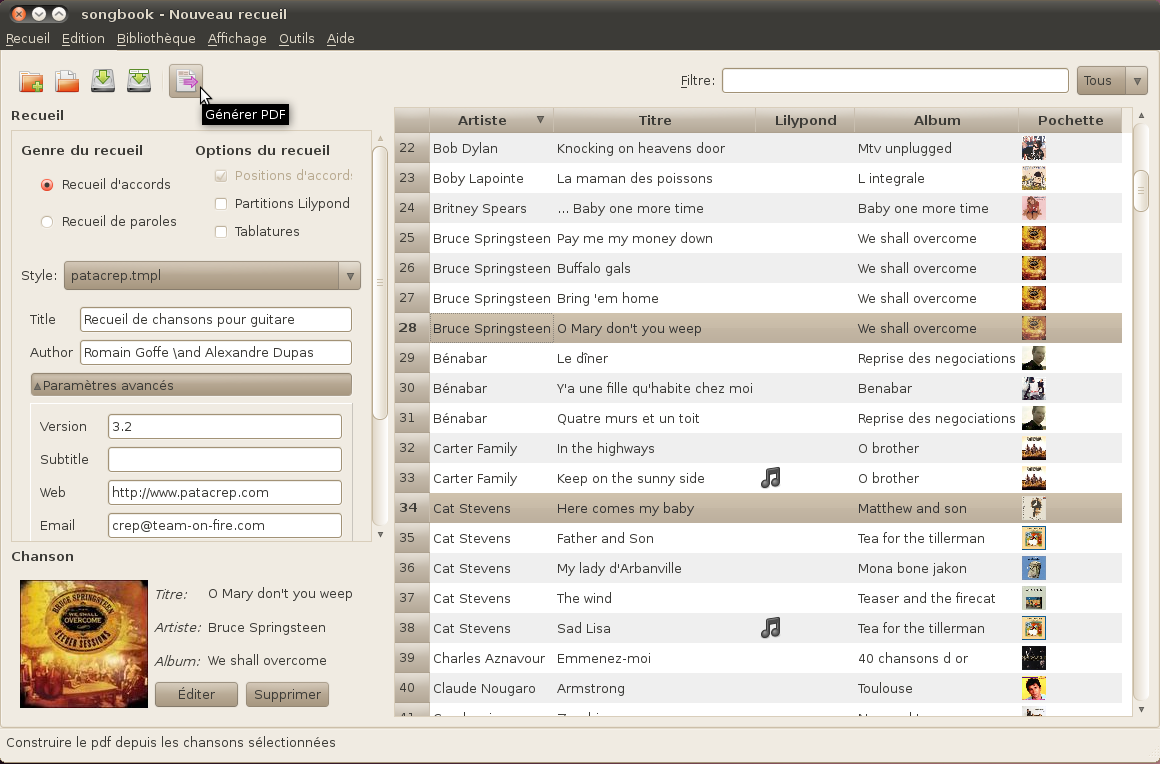
\includegraphics[width=\textwidth]{sbc-v0-3-01}
  \caption{Patacrep Songbook Client: interface pour la génération de
    recueils de chansons.}
  \label{fig:sb-client}
\end{figure}

\paragraph{Récupérer la liste des chansons}
Si vous avez installé git, vous pouvez à utiliser le menu
Bibliothèque/Download pour récupérer l'ensemble des chansons
disponibles sur \url{www.patacrep.com}. Une fois que le téléchargement
s'est bien déroulé, n'oubliez de vérifier que le chemin indiqué dans
le menu Édition/Préférences est correct et faîtes éventuellement
Bibliothèque/Refresh pour être sûr d'être correctement synchronisé
avec les fichiers .sg.

\paragraph{Sélection des chansons}
Cliquez sur les chansons que vous souhaitez voir apparaitre dans votre
recueil.  Les chansons sélectionnées sont en surbrillance. Utilisez
l'action \Touche{Générer PDF} pour générer le pdf disponble depuis le
menu Recueil/Générer ou depuis le bouton à droite dans la barre
d'outils .

\paragraph{Enregistrez votre recueil}
Un recueil est un fichier .sb dans lequel sera enregistré la liste des
chansons sélectionnées ainsi que les options et les champs
personnalisés du recueil lui-même.


\begin{nota} 
  Les captures d'écran et les explications sont valables pour la
  version 0.3. Comme le développement en est encore à ses débuts et
  qu'il est relativement actif, certains éléments sont amenés à
  changer rapidement. N'hésitez pas à demander des conseils sur le
  forum.
\end{nota}

%------------------------------------------------------------------------------
\subsection{Installation depuis les sources}
%------------------------------------------------------------------------------

\begin{nota}
  Il est nécessaire d'avoir installé au préalable les dépendances du
  songbook lui-même (voir la section
  \voir{sec:songbook-dep}{correspondante}). Pour que tous les éléments
  de l'interface fonctionnent, les dépendances recommandées sont
  \emph{fortement} recommandées.
\end{nota}

\paragraph{Dépendances}
\begin{unixcom}
  sudo apt-get install build-essential cmake
  sudo apt-get install qt4-qmake qt4-dev-tools libqt4-sql-sqlite
\end{unixcom}

\paragraph{Installation}
\begin{unixcom}
  cd $HOME
  git clone git://github.com/crep4ever/songbook-client.git
  cd songbook-client
  make
  sudo make install
\end{unixcom}
%$
%------------------------------------------------------------------------------
\subsection{Installation depuis le paquet Debian}
%------------------------------------------------------------------------------

Un paquet Debian (.deb) est disponible pour faciliter le processus
d'installation du songbook-client. 

\begin{unixcom}
  cd $HOME
  wget http://www.patacrep.com/files/songbook-client-0.3-1_amd64.deb
  sudo dpkg -i songbook-client-0.3-1_amd64.deb
\end{unixcom}
%$

\begin{nota}
  Si le lien n'est pas à jour ou si vous êtes sur une architecture
  32bits, allez dans le répertoire
  \url{http://www.patacrep.com/files/} et récupérez le fichier .deb
  adéquat.
\end{nota}

%------------------------------------------------------------------------------
\subsection{Configuration}
%------------------------------------------------------------------------------

Pour lancer l'application,
faites \Touche{Alt}+\Touche{F2} \command{songbook-client} ou dans un
terminal:
\begin{unixcom}
  songbook-client
\end{unixcom}

Une fois l'application lancée, il est important:
\begin{itemize}
\item d'indiquer le chemin du songbook dans les préférences (par
  exemple \colarg{/home/user/songbook}). Ce répertoire devant impérativement
  contenir le makefile et le répertoire \colarg{songs/} avec les chansons
  disponibles;
\item de resynchroniser la base de données avec le nouveau répertoire
  indiqué (Fichier/Synchroniser).
\end{itemize}

\begin{nota}
  La synchronisation est à utiliser dès lors que vous modifiez le
  contenu du répertoire \colarg{songs/} lorsque vous rajoutez un nouveau
  fichier (chanson, image) ou lorsque vous déplacez le répertoire
  \colarg{songbook/}.  Il n'est pas nécessaire de synchroniser si vous
  avez simplement édité un fichier (correction, \dots\,).
\end{nota}

%------------------------------------------------------------------------------
\subsection{Problèmes divers}
%------------------------------------------------------------------------------

N'hésitez pas à faire remonter les bugs que vous pouvez rencontrer sur
le forum ou par mail directement.

\paragraph{Sqlite} 
Si vous voyez une boîte de dialogue d'avertissement se lancer au
démarrage de l'application indiquant que le support de sqlite est
nécessaire, vous ne pourrez pas utiliser l'interface. Vérifiez que
votre système dispose bien du support Qt de sqlite.

\paragraph{Pas de partitions}
Si la compilation de votre recueil de chansons n'intègre pas les
partitions malgré l'option \emph{Lilypond} correctement cochée dans les
préférences, vérifiez que Lilypond est bien installé sur votre système. 

\paragraph{Liste des chansons vide} 
Vérifiez que le chemin d'accès au patacrep songbook est correctement
renseigné dans Édition/Préférences.  Le chemin indiqué doit contenir
impérativement le makefile et le répertoire \colarg{songs/}.

\paragraph{Erreurs après renommage/suppression d'une chanson} 
Un ``make clean'' ou, depuis l'interface, Songbook/Nettoyer devrait
régler le problème. S'il persiste encore, une solution radicale
consiste à supprimer manuellement tous les fichiers ``.d'' présents
dans $\sim$/songbook.


%*******************************************************************************
\section{Comment écrire une chanson}
%*******************************************************************************

%------------------------------------------------------------------------------
\subsection{À propos de \LaTeX\,}
%------------------------------------------------------------------------------

\LaTeX\, est un logiciel de traitement de texte qui va générer un
document pdf depuis un fichier source (un simple fichier texte). Cela
permet à l'utilisateur de se concentrer sur le contenu plutôt que sur
la forme. Pour que \LaTeX\, puisse produire un rendu correct, la
rédaction d'un fichier source doit respecter certaines contraintes
basées sur l'utilisation de commandes.

Une commande commence part un antislash ($\backslash$) suivi du nom de
la commande. Ensuite viennent les arguments, s'il y en a, entre
accolades (obligatoires) ou crochets (optionnels).


%------------------------------------------------------------------------------
\subsection{Éléments principaux}
%------------------------------------------------------------------------------

Une chanson est un simple fichier texte \colarg{chanson.sg} que l'on
place dans le répertoire \colarg{songs/Artiste}. Les espaces n'étant
pas tolérés, veillez à utiliser des underscores. L'entête d'un fichier
.sg se présente de la manière suivante:

\begin{verbatim}
    \beginsong{Titre}
              [by=Artiste,cov=album-cover]
\end{verbatim}

Les paramètres \command{Titre}, \command{Artiste} et
\command{album-cover} sont à renseigner pour chaque nouvelle
chanson. \command{album-cover} désigne un fichier
\colarg{album-cover.jpg} devant se trouver dans le même répertoire que
le fichier .sg.  La chanson se compose d'une succession de couplets
(verse en anglais) et de refrains (chorus). Un couplet est alors
encadré par les balises \latexcom{beginverse} et
\latexcom{endverse}. De la même manière, un refrain se trouve entre
les balises \latexcom{beginchorus} et \latexcom{endchorus}.  Les
paroles sont écrites normalement entre le \latexcom{begin} et le
\latexcom{end}. Pour préciser sur quelle syllabe un accord doit être
joué, on utilise une commande spéciale. Par exemple, la commande
\latexcom{[Mi]} produira un \command{Mi} au dessus de la syllabe
suivante. Vous pouvez utiliser n'importe quel texte pour désigner un
accord.

\begin{center}
\begin{verbatim}
\beginverse
His \[Rém]steely skin is covered
By \[Fa]centuries of dust
\[Do]Once he was a great one
\[Rém]Now he's dull and rust
\endverse
\end{verbatim}
\end{center}

Chaque chanson se termine avec la commande \latexcom{endsong}.

%------------------------------------------------------------------------------
\subsection{Règles de style}
%------------------------------------------------------------------------------

\paragraph{Notation des accords}
La convention de nommage des accords du recueil n'est \emph{pas} la
convention anglo-saxone désignation des accords par (A, B, C, D, E, F,
G) mais la notation latine (La, Si, Do, Ré, Mi, Fa, Sol). Par défaut,
l'accord est majeur (Do fait référence à l'accord de Do majeur). Les
accords mineurs sont précisés par un \command{m} minuscule.  Le
symbole bémol ($\flat$) est représenté en utilisant le caractère
\command{\&}.  Le dièse ($\sharp$) est codé par le caractère
\command{\#}. Les autres notations sont simplement ajoutées comme des
caractères à l'accord principal. Par exemple, l'accord de \command{La
  bémol mineur} est noté \latexcom{[La\&m]}.

\paragraph{Répétition des accords}
De façon à avoir un document lisible et relativement compact, les
accords des couplets et des refrains ne sont renseignés qu'une seule
fois à leur première occurence. En effet, même si jouer les morceaux
du premier couplet en chantant les paroles du second peut demander un
peu de gymnastique, cela fera travailler votre mémoire tout en offrant
un texte bien moins surchargé et (beaucoup) moins de pages à imprimer.

\paragraph{Typographie}
Chaque ligne commence par une majuscule. La ponctuation en fin de
ligne est laissée au choix de celui qui transcrit la chanson.  Les
signes composés ``; : ! ?'' prennent une espace avant en français,
mais pas en anglais. Les majuscules s'accentuent. On écrit : ``À
bientôt.'' et non pas ``A bientôt.''.

\paragraph{Numérotation des couplets et Sauts de ligne}
La numérotation se fait automatiquement pour chaque
\latexcom{beginverse} rencontré. Cependant, il est parfois plus
lisible de scinder un couplet en deux parties, la deuxième partie ne
devant pas être numérotée. Pour cela on utilise la commande
\latexcom{beginverse*}. Par exemple, un couplet en huit strophes se
décompose souvent en $2 \times 4$ strophes comme dans l'exemple
suivant.

\begin{verbatim}
\beginverse
His \[Rém]steely skin is covered
By \[Fa]centuries of dust
\[Do]Once he was a great one
\[Rém]Now he's dull and rust
\endverse

\beginverse*
An oily tear he's crying
Can you feel the pain
Of the sad, sad robot
And it's driving him insane
\endverse
\end{verbatim}

\paragraph{Agencement en colonnes}
La commande \latexcom{songcolumns} détermine le nombre de colonnes sur
lequel sera présentée la chanson. Elle s'utilise juste avant la
commande \latexcom{beginsong}. Vous pouvez indiquer le nombre de
colonnes à utiliser pour écrire votre chanson (généralement 1, 2 ou
3). Par convention, utilisez 2 colonnes par défaut.

\begin{verbatim}
\songcolumns{2}
\beginsong{Titre}
\end{verbatim}

\paragraph{Caractères spéciaux}
Quelques caractères doivent être codés différemment en utilisant des
commandes \LaTeX\, pour un meilleur résultat. Les deux exemples
principaux sont les 3 points (\dots) et le caractère \oe{}. Pour
représenter ces caractères, vous devez utiliser respectivement les
commandes \latexcom{dots} et \latexcom{oe\{\}} (ou utiliser le
caractère utf-8 \command{œ}). On utilise des accolades autour des
commandes de sorte que les commandes puissent être insérées où vous le
désirez sans interférer avec le reste du texte. Voir aussi la section
\voir{sec:utilitaires}{utilitaires}.

\paragraph{Ch\oe{}urs et répétitions}
Lorsqu'une phrase ou un couplet est répété plusieurs fois d'affilée,
utiliser la commande \latexcom{rep} plutôt que d'écrire \emph{bis} ou
d'indiquer directement (x4). Pour faire répéter quatre fois une
strophe, utilisez la commande suivante à la fin de la ligne. La
commande \latexcom{echo} fait référence à des chœurs (ou similaire).

\begin{verbatim}
Hallelujah \echo{Hallelujah} \rep{4}
\end{verbatim}


\paragraph{Diagrammes des accords}
Étant donné qu'un accord de guitare peut se jouer de plusieurs façons
différentes et qu'il est parfois judicieux de privilégier telle ou
telle position, le songbook permet de représenter schématiquement ces
accords en début de chanson. On utilise la commande \latexcom{gtab}
juste avant le premier couplet ou refrain. Voici quelques exemples
classiques:

\begin{verbatim}
\gtab{Ré}{XX0232}
\gtab{Mi}{022100}
\gtab{Do}{3:002220}
\end{verbatim}

\begin{itemize}
\item les 6 chiffres correspondent aux 6 cordes de la guitare
  (\command{Mi}, \command{La}, \command{Ré}, \command{Sol},
  \command{Si}, \command{Mi});
\item la valeur du chiffre indique la fret (case) sur laquelle on
  appuie;
\item 0 désigne une corde jouée à vide;
\item X indique que la corde ne doit pas être jouée;
\item une valeur avant un ``:'' désigne un barré: \emph{3:} indique un
  barré de trois frets.
\end{itemize}

%------------------------------------------------------------------------------
\subsection{Exemple complet}
%------------------------------------------------------------------------------

Voici un exemple complet pouvant être utilisé comme point de départ
pour écrire une nouvelle chanson.

\begin{verbatim}
\songcolumns{2}
\beginsong{Sad robot}
  [by=Pornophonique,cov=8-bit-lagerfeuer]

  \cover
  \gtab{Rém}{XX0231}
  \gtab{Fa}{1:022100}
  \gtab{Do}{X32010}

  \lilypond{Sad_robot}

  \beginverse
    His \[Rém]steely skin is covered
    By \[Fa]centuries of dust
    \[Do]Once he was a great one
    \[Rém]Now he's dull and rust
  \endverse

  \beginverse*
    An oily tear he's crying
    Can you feel the pain
    Of the sad, sad robot
    And it's driving him insane
  \endverse

  \beginverse*
    He can't turn back time nor history
    So his life became a misery
    He has to face the destiny
    Nobody cares anymore
  \endverse

  \beginchorus
    Sad, sad robot
    Sad, sad robot
    Sad, sad robot
    All alone
  \endchorus

  \beginchorus
    He's a sad, sad robot \rep{3}
    He's so alone
  \endchorus

  \beginverse
    Me steely skin is covered
    By centuries of dust
    Once me was a great one
    But now I'm dull and rust
  \endverse

  \beginverse*
    An oily tear I'm crying
    Can you feel me pain
    I'm the sad, sad robot
    Driving me insane
  \endverse

  \beginverse*
    I can't turn back time nor history
    So me life became a misery
    I have to face me destiny
    That I'm all on me own
  \endverse

  \beginchorus
    Red, red robot
    I'm a red, red robot \rep{2}
    And so I shall return
  \endchorus

  \beginchorus
    I'm a red, red robot \rep{3}
    So I shall return
  \endchorus

\endsong
\end{verbatim}

%*******************************************************************************
\section{Contribuer au projet}
%*******************************************************************************

Il est facile de contribuer au projet :

\begin{itemize}
\item signalisation des fautes d'orthographe, de musique;
\item proposition sur le forum des chansons que vous aimeriez voir transcrites;
\item transcription complète d'une chanson;
\item transcription partielle d'une chanson avec uniquement les paroles;
\item transcription Lilypond de certains solos;
\item correction de bugs, amélioration du code;
\end{itemize}

Si vous rajoutez une chanson, n'oubliez pas de nous l'envoyer et nous
serons ravis de l'intégrer. Comme toujours les contributeurs sont plus
que bienvenus. Pour nous contacter:

\begin{itemize}
\item envoyez directement vos remarques par mail à
  \url{crep@team-on-fire.com};
\item utilisez le forum comme bon vous semble;
\end{itemize}


%-------------------------------------------------------------------------------
\subsection{Création d'un patch}
%-------------------------------------------------------------------------------

Une bonne façon de nous faire remonter vos corrections/modification
est de nous les envoyer sous forme de patch. Techniquement, un patch
est un simple fichier qui indique les opérations (ajout/suppression)
qui ont été opérées sur un fichier texte. Un exemple tout simple a
l'aspect suivant:

\begin{verbatim}
index 3fcce15..b4edcc1 100644
--- a/songs/Cat_Stevens/The_wind.sg
+++ b/songs/Cat_Stevens/The_wind.sg
@@ -7,7 +7,7 @@

-\[Do] I listen to the \[Fa]wind,
    +\[Ré] I listen to the \[Sol]wind,
\end{verbatim}

Vous voyez rapidement qu'après les premières lignes qui servent à
identifier le fichier sur lequel on a travaillé, on a remplacé:
\begin{verbatim}
-\[Do] I listen to the \[Fa]wind,
\end{verbatim}
par
\begin{verbatim}
+\[Ré] I listen to the \[Sol]wind,
\end{verbatim}

Concrètement, si vous avez suivi la procédure d'installation, vous
devriez avoir un répertoire \colarg{\$HOME/songbook/} contenant toutes
les sources du carnet de chant. Maintenant, vous avez repéré une
erreur dans la chanson \colarg{songs/artiste/chanson.sg}. Ouvrez le
fichier correspondant avec votre éditeur de texte préféré, faîtes
votre correction, enregistrez, fermez. Puis, dans un terminal:

\begin{unixcom}
  cd $HOME/songbook
  git diff -u songs/artiste/chanson.sg > patch
\end{unixcom} 
%$

Cela va vous créer un nouveau fichier \colarg{patch} qui contiendra
l'ensemble des modifications que vous avez apportées à votre
chanson. Plus qu'à nous l'envoyer !

%-------------------------------------------------------------------------------
\subsection{Création de votre version du songbook}
%-------------------------------------------------------------------------------

Si vous prévoyez de faire beaucoup de modifications ou de rejoindre
activement le développement du songbook, le système de patch n'est pas
forcément adapté et il vaut mieux dans ce cas partir sur votre propre
version du songbook. La meilleure solution consiste à faire un
\emph{fork} du projet Git et de l'héberger sur le web si vous comptez
le partager. Des solutions web gratuites permettent d'héberger de tels
projets. Par exemple:

\begin{itemize}
\item \url{http://github.com}
\item \url{http://gitorious.org}
\end{itemize}

Il suffit alors de nous communiquer l'adresse de votre dépôt Git de
façon à ce que nous puissions récupérer vos changements.


%%*******************************************************************************
%\section{Accords usuels}
%%*******************************************************************************
%
%%------------------------------------------------------------------------------
%\subsection{Accords majeurs}
%%------------------------------------------------------------------------------
%
%
%%------------------------------------------------------------------------------
%\subsection{Accords mineurs}
%%------------------------------------------------------------------------------
%
%
%%------------------------------------------------------------------------------
%\subsection{Accords de 7ème}
%%------------------------------------------------------------------------------


%*******************************************************************************
\section{Partitions avec Lilypond}
%*******************************************************************************

%------------------------------------------------------------------------------
\subsection{Lilypond}
%------------------------------------------------------------------------------

La documentation du projet Lilypond est très
claire et se trouve sur le site \url{http://lilypond.org/}.
Voici néanmoins quelques concepts de base:

\begin{itemize}
\item les lettres a, b, c, d, e, f, g représente les notes la, si, do,
  ré, mi, fa, sol;
\item un chiffre derrière une lettre en indique la durée (2=blanche, 4=noire,
  8=croche) et un point après un chiffre désigne une note pointée;
\item \emph{ais}, \emph{bes} désignent un \emph{la dièse} et un \emph{si bémol}
\item \emph{'} et \emph{,} servent à monter/descendre d'une octave;
\end{itemize}

Lilypond est généralement empaqueté pour les distributions
GNU/Linux. Pour des distributions basées Debian/Ubuntu, l'installation
se fait par:

\begin{unixcom}
  sudo apt-get install lilypond
\end{unixcom}


%------------------------------------------------------------------------------
\subsection{Intégration au songbook}
%------------------------------------------------------------------------------

Si vous voulez rajouter une ligne mélodique dans une chanson, vous
pouvez utiliser lilypond pour générer la partition. Créez pour cela un
nouveau fichier \colarg{partition.ly} dans le répertoire
\colarg{songbook/lilypond}.  Il faut inclure le fichier d'en-tête
\colarg{header} et définir l'option paper-height de façon à ce que la
partition produite tienne sur une page avec le moins de blanc
possible. Une première estimation est de compter 1.6cm pour une
ligne. Puis, écrivez votre partition entre accolades comme dans
l'exemple suivant (Tom Sawyer) pour obtenir le résultat en
Fig.~\ref{fig:lilypond}:

\begin{verbatim}
\include "header"
\paper{paper-height = 3.3\cm}
 {
   \key c \major
   \time 2/4
   \relative c''{
     e4 c g'2 a4 a8. a16 g8 e4 c8 a'4 a8. a16 g8 f e c d2~ d4
     e8 f g4 g8. g16 f8 e d c a c4 a8 g4 c8 d e8 g4 g,8 e' e d d c2
   }
 }
\end{verbatim}

\begin{figure}
  \centering
  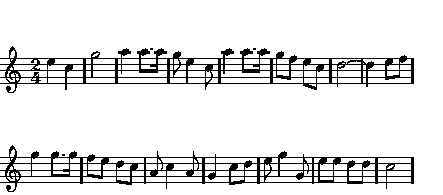
\includegraphics[width=0.8\textwidth]{lilypond}
  \caption{Intégration de partitions avec Lilypond.}
  \label{fig:lilypond}
\end{figure}

Enfin, pour insérer votre partition dans une chanson, insérez la ligne
suivante à l'endroit désiré dans \colarg{chanson.sg}:

\begin{verbatim}
\lilypond{partition}
\end{verbatim}

Toutes les partitions lilypond présentes dans le répertoire
\colarg{songbook/lilypond} sont automatiquement générées par le
makefile. Pour construire le songbook incluant les partitions
lilypond, il suffit de faire:

\begin{unixcom}
  make lilypondbook.pdf 
\end{unixcom}

\begin{nota}
  Auparavant, il était nécessaire de générer au préalable les
  partitions lilypond avec la commande ``make lilypond''. Cette étape
  n'est désormais plus nécessaire, le makefile génèrera
  automatiquement les paritions lilypond nécessaires.
\end{nota}

%*******************************************************************************
\section{Utilitaires}
\label{sec:utilitaires}
%*******************************************************************************

Des scripts utilitaires sont disponibles dans le répertoire
\colarg{songbook/utils}. On les exécute classiquement en faisant:

\begin{unixcom}
  cd $HOME/songbook
  ./utils/script.sh
\end{unixcom}
%$

\paragraph{Resize cover}
Permet de redimensionner automatiquement tous les fichiers .jpg du
répertoire \colarg{songbook/songs} correspondant aux pochettes des
albums. À exécuter après l'ajout d'une nouvelle pochette jpg.

\paragraph{Latex preprocessing}
Applique un ensemble de règles automatiques pour les notations
\LaTeX\, de certains caractères et pour les notations d'accords.  À
exécuter après l'ajout d'une nouvelle chanson pour être sûr de
respecter les standards du songbook.

\paragraph{New songs list}
Permet de récupérer la liste des chansons ajoutées depuis la dernière
version.

\paragraph{Volume\,2}
Permet de générer la liste des chansons qui ne sont pas dans le
volume\,1.

\paragraph{Make html}
Génère la liste de toutes les chansons au format html.


%*******************************************************************************
\section{Conseils aux débutants}
%*******************************************************************************

%------------------------------------------------------------------------------
\subsection{Les accords de base}
%------------------------------------------------------------------------------

Les accords de base sont les accords qui se jouent sans barré au
niveau des premières frets:

\begin{itemize}
\item Accords Majeurs:\\ \command{Do} (X32010), \command{Sol}
  (320003), \command{La} (X02220), \command{Ré} (XX0232), \command{Mi}
  (022100)\\
\item Accords Mineurs:\\
  \command{Mim} (022000), \command{Lam} (X02210), \command{Rém} (XX0231)\\
\item Accords Septième:\\ \command{Mi7} (020100), \command{Sol7}
  (320001), \command{Ré}7 (XX0212), \command{La7} (X02020),
  \command{Si7} (X21202)\\
\end{itemize}

Donc déjà, il est bon de savoir jouer et enchainer assez rapidement
ces accords là. Le mieux c'est de chercher des morceaux avec ces
accords et de s'entraîner dessus.  À part dans certains cas comme pour
l'accord de \command{Ré}, les cordes marquées d'un X peuvent quand
même sonner.  C'est juste qu'on préfère généralement attaquer par la
fondamentale de l'accord (ex: note \command{Do} pour l'accord de
\command{Do majeur}). À propos des différentes notations d'accords,
il s'agit juste d'une question de sonorité ou de pragmatisme. On est
toujours libre de jouer l'accord de la façon qui nous arrange le plus.

%------------------------------------------------------------------------------
\subsection{Transposer un morceau}
%------------------------------------------------------------------------------

L'idée, c'est de toujours pouvoir se ramener à un enchaînement
d'accords que l'on maîtrise.  Pour transposer un morceau, c'est pas
dur il suffit d'appliquer le même décalage à tous les accords.  Par
exemple, pour la chanson du hérisson, si on décale de 2 tons 1/2:
\command{Sim}, \command{Sol}, \command{Fa$\sharp$7} se transposent en
\command{Mim}, \command{Do}, \command{Si7}.  Et miracle, ces
accords-là ne demandent plus de barrés !

%------------------------------------------------------------------------------
\subsection{Les barrés}
%------------------------------------------------------------------------------

Bon, le coup de transposer les accords, c'est un bon exercice pour
jongler avec les accords et leurs enchaînements mais de temps en
temps, ça ne suffit pas, il reste toujours des barrés qui apparaissent
et c'est quand même mieux de jouer les vrais accords. Donc attaquons
la fameuse technique du barré. Tout bon débutant qui se respecte
commence par le barré de \command{Mi} \dots\, pour faire un
\command{Fa}. Oui, en fait, un barré, c'est se servir de son index comme
capo pour transposer l'accord qu'on fait dessous (avec un doigt en
moins).

Exemple: l'accord de \command{Fa} se joue 133211. Il est cependant
noté 1:022100 dans le carnet de chant car c'est un barré de
\command{Mi} (022100) sur la première fret.  Donc l'idée, c'est
d'appuyer bien fort avec son index en travers de toutes les cordes et
d'utiliser annulaire, ptit doigt, majeur pour appuyer sur les 3 cordes
demandées. À savoir qu'il y a essentiellement 4 types de barrés.  Dans
l'ordre de difficulté: barrés de \command{Mi} (022100), \command{Lam}
(002210), \command{Mim} (022000), \command{La} (002220).

%------------------------------------------------------------------------------
\subsection{Les rythmes}
%------------------------------------------------------------------------------

Contrairement à ce que l'on pourrait croire, il est bien plus
difficile de maîtriser la main droite que la main gauche.
Voici quelques motifs assez passe-partout pour vos morceaux.

\paragraph{Rythme ``à la Brassens''} Il s'agit d'alterner une basse (pouce)
avec 3 aiguës simultanées (index, majeur, annulaire), 2 ou 4 fois par
accord. En général, les 3 aiguës sont les 3 cordes aiguës 4,5,6
(\command{Sol}, \command{Si}, \command{Mi}) et la basse alterne entre
les cordes 1,2,3 (\command{Mi}, \command{La}, \command{Ré}) mais
souvent dans l'ordre 2,1.

\paragraph{Rythme ``arpège''} Il s'agit d'un motif note-à-note qui
accompagne très bien les chansons calmes. Chaque guitariste a le
sien, voici l'ordre des cordes à jouer pour le mien: 2~654~654~6. En
gros, on fait une basse avec le pouce, puis deux descentes aiguës avec
annulaire, majeur, index et on finit par la plus aiguë.

\paragraph{Rythme ``feu de camp''} Quand il faut gratter, le premier
piège est de suivre le rythme du chant. Gardez un rythme constant !
//arf, j'arrive pas à expliquer ... //


%------------------------------------------------------------------------------
\subsection{Les techniques du fourbe}
%------------------------------------------------------------------------------

Alors je ne sais pas trop si ça peut aider ou non mais j'ai mis au
point mes propres techniques secrètes de débutant feignant. Elles sont
quand même relativement déconseillées dans la mesure où ce sont de
mauvaises habitudes pas académiques dont on a du mal à se défaire.

\paragraph{L'accord de \command{Sol}}
Arf, voilà mon premier échec à la guitare. Après avoir enchainé des
accords de \command{La} et de \command{Mi} pendant 3 heures je
m'essaye au \command{Sol}. Position ok, ça sonne bien. Manque de pot,
impossible d'enchainer ça rapidement.  Du coup, remarquant qu'un
\command{Sol} se jouait en 320003, je me suis dit qu'avec un seul
doigt, j'avais déjà 4 cordes sur 6. Donc j'ai commencé en jouant mes
\command{Sol} en XX0003 avec seulement l'annulaire et ça sonnait très
bien. Un an plus tard, j'ai réalisé qu'en mettant le pouce sur la
première corde, ça marchait encore mieux (3X0003) donc voilà la
technique de la pince pour l'accord de Sol qui fait beaucoup rire les
vrais guitaristes quand ils me voient jouer.

\paragraph{L'accord de \command{Fa}}
Après avoir contourné le problème du \command{Sol} s'est posé celui du
\command{Fa}. Là c'est pareil, impossible de tenir la position barrée
plus de deux nanosecondes sans hurler de douleur.  Je me suis dit,
trouvons une parade: le semi barré.  En fait, quand on regarde la
théorie du barré, c'est pas bien optimisé puisque l'index appuie sur
toutes les cordes donc on appuie 2 fois sur certaines cordes (index
111111, autres doigts 033200). Donc en fin de comptes, l'index sert
seulement pour les cordes 1,5 et 6. Au diable la première, mon index
fera 5 et 6 et ce sera suffisant.  Ça donne des \command{Fa} comme ça:
X33211 avec l'index qui écrase seulement les deux dernières
cordes. Bon, autant je fais encore mes \command{Sol} avec mon pouce,
autant j'ai appris à faire des barrés proprement.

\end{document}
